% !TeX spellcheck = it_IT
\newpage
\section{Kernel}
\subsection{Booting}
Il boot è un aspetto critico messo a disposizione dalla microarchitettura: all'avvio il processore esegue il codice nella ROM per caricare il \textbf{first-stage bootloader}. Questo inizializza il controller della memoria e alcune periferiche di I/O per permettere al \textbf{second-stage bootloader} di essere caricato. Quest'utlimo carica il kernel e il filesystem, a cui poi è ceduto il controllo.
\begin{center}
	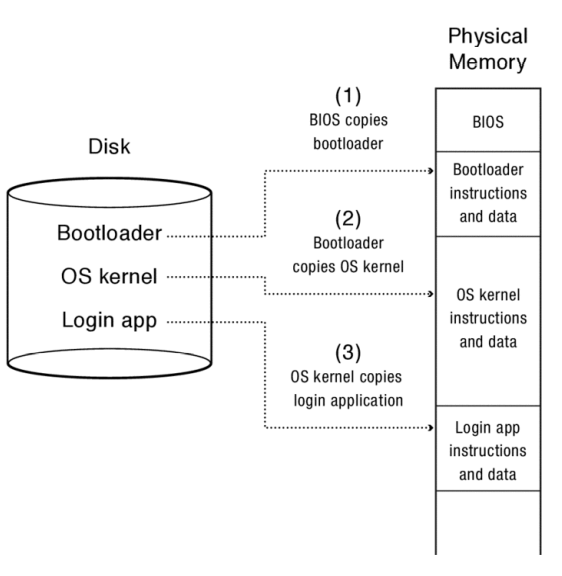
\includegraphics[scale=0.3]{kernel_boot.png}
\end{center}
\begin{note}
	Il BIOS risiede in una memoria volatile e permette di fare dei controlli basilari di sistema e caricare il bootloader. La versione moderna è lo UEFI. Si occupa anche di fare controlli di \textbf{sicurezza} per assicurarsi che il kernel caricato non sia modificato.
\end{note}
\subsection{Processi}
Un processo è una struttura dati (PCB) su cui vengono memorizzate tutte le informazioni riguardanti memoria, file aperti, sottoprocessi.
\begin{note}
	Noi faremo riferimento sempre ai sistemi UNIX che sfrutta diverse semplici chiamate. Sotto Windows la chiamata per creare i processi è molto più articolata.
\end{note}
I comandi principali su UNIX sono: \textbf{fork}, \textbf{exec}, \textbf{wait} e \textbf{signal}.
\begin{center}
	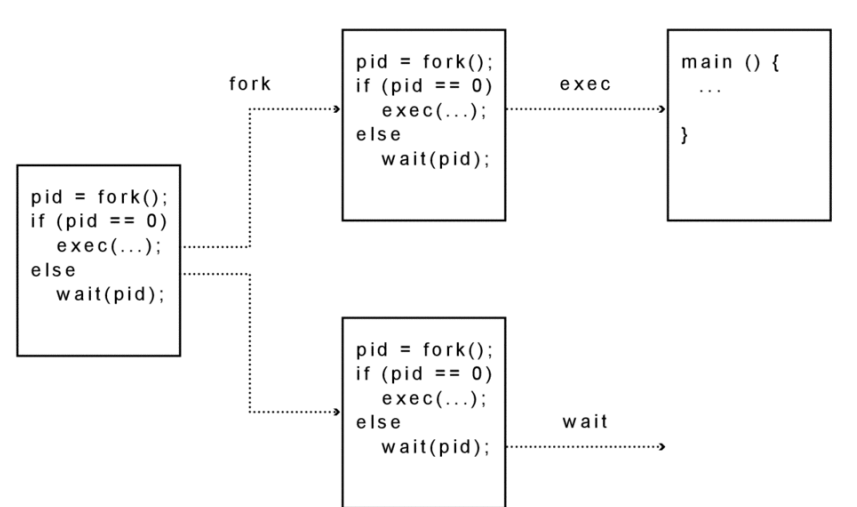
\includegraphics[scale=0.3]{process_management.png}
\end{center}

\subsubsection{Fork}
La fork crea una copia del processo corrente (\emph{figlio}) che condivide il codice e lo stack del \emph{padre}. Al processo padre restituisce l'ID del PCB del figlio (o un eventuale codice di errore), mentre al figlio restituisce 0.
\begin{note}
	Come detto in precedenza la copia del PCB non è totale tra padre e figlio, ma fatta in modo che ci siano solo le parti utilizzate, dato che è possibile che poco dopo venga sovra scritta da una \emph{exec}.
\end{note}
\noindent La \emph{fork} può \textbf{fallire} in diversi casi, ad esempio quando non c'è sufficiente memoria.\\
Quali sono i passaggi della fork?
\begin{enumerate}
	\item Creata e inizializzato il PCB nel kernel
	\item Creato un address space
	\item Viene inizializzato l'address space con una copia di tutti i contenuti dello spazio di indirizzo del padre
	\item Vengono copiati i parametri nella memoria dell'address space
	\item Viene ereditata dal padre il contesto di esecuzione (e.g. tutti i file aperti)
	\item Viene informato lo scheduler che c'è un nuovo processo attivo
\end{enumerate}
\begin{center}
	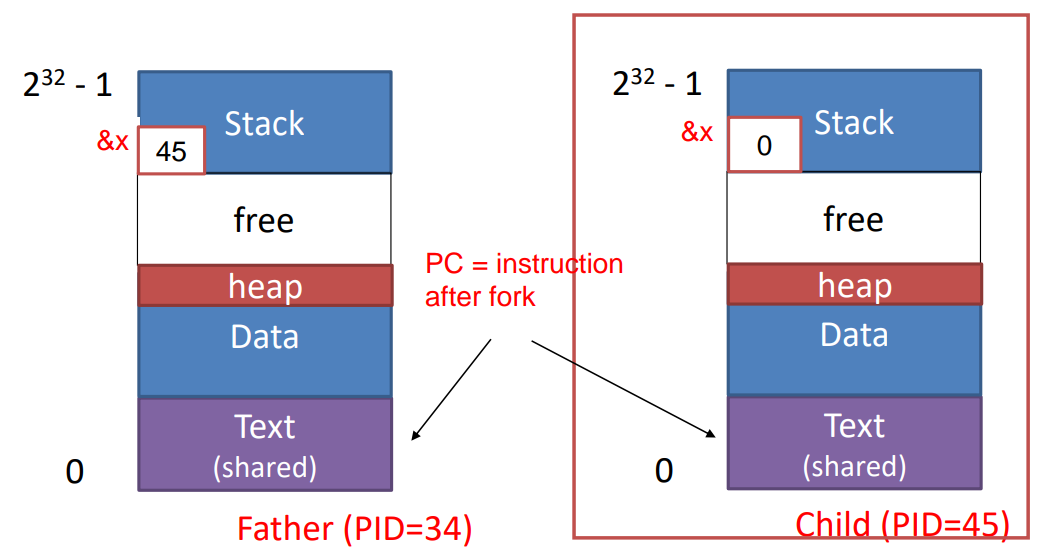
\includegraphics[scale=0.25]{fork.png}
\end{center}
\begin{example}
	Un esercizio da compitino:
	\begin{lstlisting}[language=c]
		#include <sys/types.h>
		#include <unistd.h>
		#include <stdio.h>
		
		int main(){
			fork();
			printf("Pid %d\n", getpid());
			fork();
			printf("Pid %d\n", getpid());
			
			return 0;
		}
	\end{lstlisting}
	Quanti ne stampa? 4
\end{example}

\subsubsection{Exec}
Questa chiamata sostituisce il codice eseguito da un processo, rimpiazzandone tutti i dati.
\begin{lstlisting}[language=C]
	int execl(char *pathname,char *arg0,...,char *argN, (char*)0)
\end{lstlisting}
La \emph{exec} può \textbf{fallire} (e.g. per un parametro sbagliato) ma non ritorna, dato che non ci sarebbe un codice a cui può ritornare.\\
Se invece ritorna con \textbf{successo}, il processo su cui viene eseguita mantiene il PID e il PCB, mentre resetta i \emph{pending signals}. Mantiene anche il \emph{kernel stack} e le risorse (e.g. file aperti).

\subsubsection{Terminazione}
Un processo può terminare perché ha ricevuto un'eccezione o chiamando \emph{exit}.\\ Un processo terminato restituisce il valore di ritorno al padre, che lo riceve tramite una \emph{wait}. Se quest'ultima non è ancora stata chiamata il figlio diventa \textbf{zombie}, rimanendo in attesa della chiamata o venendo eliminato dopo la morte del padre.\\
\begin{lstlisting}[language=C]
	void exit(int status);
	int wait(int *status);
\end{lstlisting}
La \emph{wait} può ritornare immediatamente ad esempio se il processo da aspettare è già terminato.
\begin{note}
	Mai fare assunzioni sulla durata dei processi. Evitare assolutamente di usare la \emph{sleep} per eseguire la sincronizzazione.
\end{note}

\subsubsection{Shell}
Un aspetto importante dei processi è la \textbf{shell}, un programma di controllo che si occupa di eseguire comandi o altri processi e di riportare sullo standard output eventuali risultati o errori.\\ Questa sfrutterà principalmente chiamate di sistema come fork, exec, waitpid, etc...\\
Un'implementazione di una shell può essere la seguente:
\begin{lstlisting}
	char *prog, **args;
	int child_pid;
	// Leggo ed elaboro l'input una riga alla volta
	while (readAndParseCmdLine(&prog, &args)) { 
		child_pid = fork(); // Creo un processo figlio
		if (child_pid == 0) {
			exec(prog, args); // Sono il processo figlio, eseguo il programma
			// Non raggiunto
		} else {
			wait(child_pid); // Sono il processo padre, aspetto il figlio
			// Controllo lo stato di uscita
		}
	}
\end{lstlisting}

\begin{note}
	Se con il codice di esempio proviamo ad eseguire il comando \emph{cd}, restituirà errore. Questo perché è implementato direttamente dalla shell e non dal sistema operativo.
\end{note}

\subsubsection{I/O Unix}
Le chiamate di sistema in Unix che si occupano dell'I/O sono \textbf{byte oriented} (non fortemente tipate). Il kernel inoltre fa della \textbf{bufferizzazione} (caricando un blocco invece che un byte), quindi \emph{fopen}, \emph{fread}, etc... sono più veloci di \emph{open}, \emph{read}, etc... mantenendo comunque l'overhead derivante dalle \emph{system call}.\\
La chiamata \textbf{open} ha diverse funzionalità e accetta molti parametri:
\begin{itemize}
	\item Se il file non esiste, restituisce un errore o lo crea
	\item Se il file esiste, restituisce un errore o apre il file
	\item Se il file esiste ma non è vuoto, lo sovrascrive e poi lo apre oppure restituisce un errore
\end{itemize}
Viene tutto fatto da una sola funzione invece che da molteplici poiché è necessario fare questo tipo di operazioni in modo \textbf{atomico}.
\begin{example}
	Nel seguente codice
	\begin{lstlisting}[language=C]
		if(|exists(name))
			create(name);
		open(name);
	\end{lstlisting}
	Tra il controllo di esistenza e la creazione, il sistema operativo potrebbe portarsi avanti ed anticipare la creazione, causando problemi.
\end{example}